\documentclass[a4paper,10pt]{article}

\usepackage[margin=2cm, tmargin=1.5in, headheight=40px]{geometry}
\usepackage[sfdefault, medium, light]{roboto}
%\usepackage[nomap]{FiraMono}
\usepackage[T1]{fontenc}
\usepackage[utf8]{inputenc}
\usepackage[spanish]{babel}
\usepackage{graphicx}
\usepackage{fancyhdr}
\usepackage{minted}
\usepackage[svgnames]{xcolor}
\setminted{style=default,bgcolor=Gainsboro}
\usepackage[allcolors={DarkSlateBlue}, colorlinks]{hyperref}

\fancyhf{}
\fancyhead[L]{
\includegraphics[height=35px]{../figuras/logoort.png}}
\fancyhead[R]{Facultad de Ingeniería \\ Cátedra de Redes y Sistemas de Comunicación}
\fancyfoot[R]{Página \thepage}
\fancyfoot[L]{Redes de Datos -- Laboratorio 3}
\renewcommand{\footrulewidth}{0.2pt}
\renewcommand{\headrulewidth}{0.2pt}

\pagestyle{fancy}


\title{\bf Redes de Datos\\Laboratorio 4 -- Capa de Red\\ Direccionamiento y ruteo estático}
\author{\bf Universidad ORT Uruguay}
\date{\bf Curso 2025}

\begin{document}

\maketitle
\thispagestyle{fancy}

En este laboratorio trabajaremos a nivel de Capa de Red, utilizando equipos Cisco disponibles en el Laboratorio. Los objetivos son:

\begin{itemize}
    \item Realizar una asignación de direcciones de una topología dada.
    \item Configurar dicha asignación en los equipos, tanto routers como hosts, de manera de implementar la capa de red.
    \item Realizar la configuración de rutas estáticas para lograr conectividad en toda la topología.
\end{itemize}

Para ello, disponemos en el laboratorio de Routers pre-cableados en topología de anillo, utilizando enlaces \textbf{seriales} punto a punto. Los routers disponen además de interfaces \textbf{Ethernet} (FastEthernet o GigabitEthernet, según el modelo). Sin embargo, los routers inicialmente tienen todas sus interfaces apagadas y sin configurar.

La topología del laboratorio es la siguiente:

\bigskip

\begin{center}
    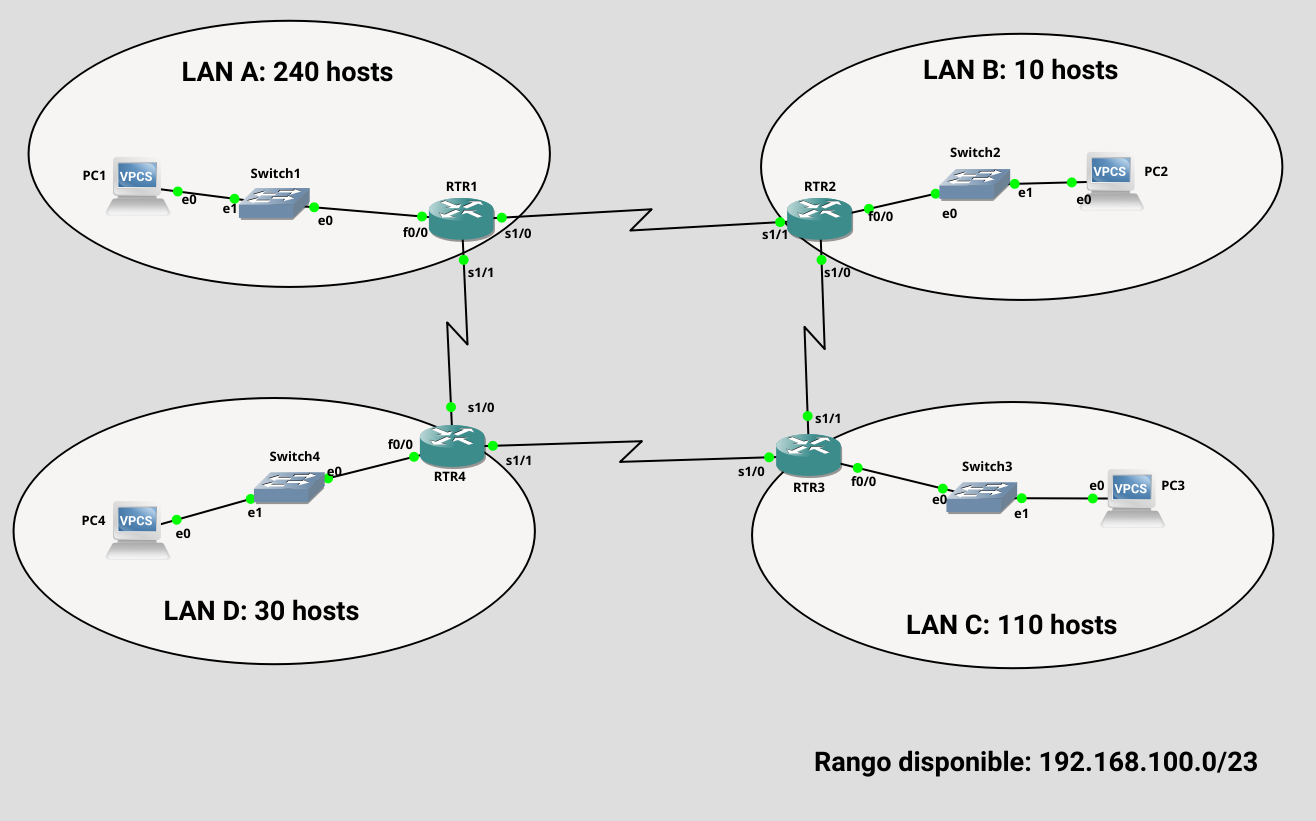
\includegraphics[width=0.85\textwidth]{../figuras/topologia_lab.png}
\end{center}

Durante la práctica, cada grupo se encargará de configurar \emph{un único router} y su LAN asociada. Sin embargo, debe coordinar con sus compañeros para que la asignación de direcciones y rutas sea \emph{coherente}.

\vfill

\section{Asignación de direcciones}

Realice una asignación de direcciones completa para las redes de área local de la figura, así como para los enlaces punto a punto entre routers, utilizando el rango provisto. Complete las siguientes tablas
    
    \begin{center}
        \bigskip
        \begin{tabular}{|p{1cm}|p{3cm}|p{3cm}|p{3cm}|p{3cm}|}
            \hline
            \textbf{Red} & \textbf{Dirección de red} & \textbf{Máscara} & \textbf{Dir. de broadcast} & \textbf{IP Router} \\ \hline
            \textbf{LAN A} & & & & \\ \hline
            \textbf{LAN B} & & & & \\ \hline
            \textbf{LAN C} & & & & \\ \hline
            \textbf{LAN D} & & & & \\ \hline
        \end{tabular}
    \end{center}

    \bigskip
    \begin{center}
        \begin{tabular}{|p{2cm}|p{2.5cm}|p{2.5cm}|p{2.6cm}|p{2.4cm}|p{2.4cm}|}
            \hline
            \textbf{Enlace} & \textbf{Dirección de red} & \textbf{Máscara} & \textbf{Dir. de broadcast} & \textbf{IP Router A} & \textbf{IP Router B} \\ \hline
            \textbf{RTR1--RTR2} & & & & & \\ \hline
            \textbf{RTR2--RTR3} & & & & & \\ \hline
            \textbf{RTR3--RTR4} & & & & & \\ \hline
            \textbf{RTR4--RTR1} & & & & & \\ \hline
        \end{tabular}
    \bigskip
    \end{center}

    Comparta la asignación realizada con el resto de los grupos de su topología de modo de llegar a una asignación coherente.

\section{Configuración de interfaces en los routers}

Para conectarse a los routers, debe accederse a los mismos mediante su \emph{consola de configuración}. Típicamente esto se realiza mediante un cable dedicado y una conexión serial. Para simplificar este proceso, en el laboratorio se dispone de un equipo Cisco remotizador de consolas. Para acceder al Router RTRX, se debe ingresar via \texttt{telnet} al remotizador, y luego acceder a la consola del Router deseado mediante:
\begin{minted}{batch}
> telnet 172.20.20.24
> Login: grupoX
> Password: ort
\end{minted}
donde X es el no. de router.

\begin{enumerate}
    \item Configure las interfaces del Router siguiendo la asignación elegida. Tenga presente el nombre de las interfaces que los conectan con Routers vecinos, disponibles en el rack del laboratorio. Puede ayudarse de los comandos en el apéndice.
    \item Verifique el estado de las interfaces mediante el comando \texttt{show ip interface brief}.
    \item Verifique el estado inicial de la tabla de rutas mediante el comando \texttt{show ip route}.
    \item Verifique conectividad a los routers directamente conectados mediante el comando \texttt{ping <IP>}.
\end{enumerate}

\section{Conexión de máquinas de usuario}

\begin{enumerate}
    \item Implemente la red local conectando un Switch a la interfaz Ethernet del router. Verifique que ahora la misma queda activa.
    \item Conecte su máquina del laboratorio a dicha red mediante un patch-cord adecuado, utilizando la tarjeta de red secundaria de la máquina.
    \item Configure la dirección IP, máscara y puerta de enlace predeterminada de su máquina para que quede conectada a la LAN adecuada.
    \item Chequee conectividad con el Router mediante \texttt{ping}. ¿Puede llegar más allá?
\end{enumerate}

\section{Implementación de rutas estáticas}

\begin{enumerate}
    \item Configure las rutas estáticas adecuadas en su router para que toda la red sea alcanzable.
    \item Si ud. configura su Router, pero los vecinos aún no, ¿enviar un \texttt{ping} entre dos hosts será posible? ¿Por qué?
    \item Una vez configurada toda la topología, verifique conectividad a toda la red.
\end{enumerate}


\appendix

\section{Comandos Cisco}

\begin{itemize}
    \item Ingresar al modo administrador:
\mintinline{batch}{RTRX> enable}
    \item Mostrar la configuración actual:
    \mintinline{batch}{RTRX# show running-config}
    \item Mostrar las interfaces (resumen): \mintinline{batch}{RTRX# show ip interface brief}
    \item Mostrar la tabla de rutas:
    \mintinline{batch}{RTRX# show ip route}
    \item Entrar al modo configuración: \mintinline{batch}{RTRX# configure terminal}
    \item Entrar a la conf. de interfaz (ej: FastEthernet 0/0): \mintinline{batch}{RTRX(config)# interface FastEthernet 0/0}
    \item Asignar IP a una interfaz: \mintinline{batch}{RTRX(config-if)# ip address <IP> <mascara>}
    
    donde la IP y la máscara van en formato decimal separadas por puntos.
    \item Asignar IP de broadcast: \mintinline{batch}{RTRX(config-if)# ip broadcast-address <IP>}
    \item Crear una ruta estática: \mintinline{batch}{RTRX(config)# ip route <dir. Red> <máscara> <nextHop>}
    \item Salir de un submenú: \mintinline{batch}{RTRX(config)# exit}

\end{itemize}
\end{document}